%%%%%%%%%%%%%%%%%%%%%%%%%%%%%%%%%%%%%%%%%%%%%%%%%%%%%%%%%%%%%%%%%%%%%%%%
\chapter{Vergleich}
\label{sec:comparison}
%%%%%%%%%%%%%%%%%%%%%%%%%%%%%%%%%%%%%%%%%%%%%%%%%%%%%%%%%%%%%%%%%%%%%%%%
Es folgt nun eine Gegenüberstellung der einzelnen Frameworks, anhand der in Kapitel \ref{sec:methodik} definierten Kriterien. Als erster wird ein genereller Überblick über die einzelnen Fakten zu den Frameworks gegeben und deren Unterschiede hervorgehoben. Danach wird noch genauer auf relevanten Kriterien für das Revex Projekt eingegangen.

\section{Gegenüberstellung der Frameworks}

\textbf{Entwicklungskultur rund um die Frameworks}\\
Alle Frameworks werden unter einer Open Source Lizenz zur Verfügung gestellt. Einige Lizenzen beinhalten aber ein Copyleft, was verlangt, dass die entwickelte Software ebenfalls wieder unter der gleichen Lizenz als \acrfull{OSS} zur Verfügung gestellt wird. Die wichtigste Copyleft-Lizenz ist die \acrfull{GPL}. Die GPL bestimmt, dass Software, welche eine Framework unter dieser Lizenz nutzt, wiederum nur unter GPL vertrieben werden darf. Die Apache License ist eine Lizenz ohne Copyleft, es ist daher zulässig Frameworks mit dieser Lizenz in proprietärer Software zu verwenden. Die \acrfull{CDDL} beinhaltet ein abgeschwächtes Copyleft, lizenzierter Code kann in einem anderen Framework verwendet werden, solange dieser Code nicht auf Dateiebene gemischt wird. Die CDDL verbietet nicht, entwickelte Software unter einer anderen Lizenz zu veröffentlichen. Für die reinen Nutzer von OSS, welche die Frameworks weder weiterentwickeln noch vertreiben wollen, spielen die Unterschiede der verschiedenen OSS-Lizenzen kaum eine Rolle. Will ein Entwickler jedoch seine Arbeitsergebnisse nicht als OSS veröffentlichen, darf er für seine Arbeiten keine OSS Frameworks verwenden, welche mit einem strengen Copyleft lizenziert sind \cite{openSource}. Die Lizenzen der einzelnen Frameworks könnten aus der Tabelle \ref{tableVergleich} entnommen werden.
\\\\
OSS wird durch Communities entwickelt, weiterentwickelt und gewartet. Dabei übernimmt die Community zahlreiche Aufgaben, die bei Closed Software vom Hersteller oder Anbieter wahrgenommen werden. In der Regel gibt es zu jeder OSS genau eine Community. User der Software können dabei registriertes Mitglied der Community sein und aktiv am Projekt als Entwickler oder Tester mitarbeiten. Die Qualität einer Software hängt dabei maßgeblich von der Größe und der Struktur der Community ab. Sind zahlreiche aktive Mitglieder mit unterschiedlichen Rollen am Projekt beteiligt, ist dies eine Grundlage für eine gute Qualität der Software \cite{openSource:community}. Alle untersuchten Frameworks weisen eine aktive und starke Community auf.
\\\\
Um die Anwendung neuer Frameworks zu lernen, lesen 78 Prozent der Entwickler die Dokumentation, 55 Prozent verwenden Codebeispiele und 29 Prozent fragen Kollegen \cite{robillard:apis}. Dadurch ist es besonders wichtig auf eine aktuelle Dokumentation des Source-Codes Zugriff zu haben. Wird nur eine veraltete Dokumentation zur Verfügung gestellt, kann es passieren das die entwickelte Software Sicherheitslücken hat oder mehr Zeit für eine korrekte Implementierung benötigt wird \cite{lethbridge:documentation}. Für alle Frameworks ist eine aktuelle Dokumentation vorhanden. Die Dokumentation von Retrofit deckt nur die grundlegend Funktionsweise ab und ist im Vergleich zu den anderen schwächer, da diese umfangreicher und genauer sind. Es konnten auch Codebeispiele für alle Frameworks gefunden werden, diese sind gut erklärt und ermöglichen es eine lauffähige Anwendung zu implementieren. Problematisch war es allerdings die gefunden Jersey Codebeispiele unter Android zu starten, da keines dieser speziell für Android entwickelt wurde. Es musste zuerst ein Workaround (siehe Kapitel \ref{workaroundAndroid}) durchgeführt werden, um die Beispiel auf einem Android Gerät starten zu können.
\\\\
\textbf{Performance}\\
Mobile Geräte haben längst Einzug in das Alltagsleben erhalten, viele Nutzer erweitern die Funktionalität der Geräte mit zahlreichen Anwendungen. Jede installierte App auf einen mobilen Endgerät hat Einfluss auf den Energieverbrauch. Je mehr Anwendungen auf eine Endgerät installiert sind und je öfter diese genutzt werden, desto höher ist der Energieverbrauch und die Betriebszeit sinkt dadurch massiv \cite{Wil2012}. Daher ist bei der Entwicklung darauf zu achten, das der Energieverbrauch so gering wie möglich gehalten wird. Auswirkungen auf den Energieverbrauch eines Smartphones haben sowohl der Bildschirm, die \acrfull{CPU}, die Kommunikation über das Mobilfunknetz, als auch das WLAN-Modul. Werden die einzelnen Komponenten so wenig wie möglich beansprucht, ist der Energieverbrauch der Anwendung gering \cite{vetter}. 
\\\\
Umso länger und mehr Daten bei einem Request über das Mobilfunknetz oder das WLAN-Modul übertragen werden, desto mehr Energie wird verbraucht. Es sollte daher darauf geachtet werden, dass die Requestdauer möglichst gering ist und nicht unnötige Daten übertragen werden. Des weiteren ist die Rechenleistung von Smartphones  wesentlich geringer als jene von Notebooks, um die Betriebszeit zu erhöhen. Daher ist bei der Entwicklung auch darauf zu achten, dass die CPU Beanspruchung der Apps gering gehalten wird, damit das System performant weiterarbeiten kann \cite{mittal:energy}. Außerdem sollte die benötigte CPU Leistung aus einem weiteren Grund möglichst gering sein, den die Hardware variiert von Smartphone zu Smartphone. Ist die benötigte CPU Leistung gering, ist es möglich die App auf nahezu allen mobilen Geräten zu installieren und zu starten \cite{joorabchi:challenges}. 
\\\\
Für den Performance Vergleich wurden daher sowohl die CPU-Auslastung, als auch die Dauer für GET- und POST Requests (Dauer der Netzwerkkommunikation) der einzelnen Frameworks gegenübergestellt. Um Vergleichswerte zu ermitteln, wurden jede App einzeln in einem Emulator gestartet und die gleich Abfolge an Funktionsaufrufen durchgeführt. 
\\\\
Die Zeitdauer der GET-Requests bei der Abbildung \ref{getRequests} setzt sich aus 11 einzeln abgesetzte GET-Requests zusammen. Diese Requests werden benötigt, um die Details zu einem bestimmten Kraftwerke anzuzeigen. Es werden in der Praxis oft mehrere GET-Request hintereinander abgesetzt, daher wurde die Dauer ermittelt um alle Details zu einem Kraftwerk abzurufen. Es konnte dabei festgestellt werden, dass Retrofit am schnellsten ist, dicht gefolgt von AndroidAnnotations und Jersey am langsamsten ist.

\begin{figure} [ht]
	\centering
	\subfloat[GET Request Retrofit]{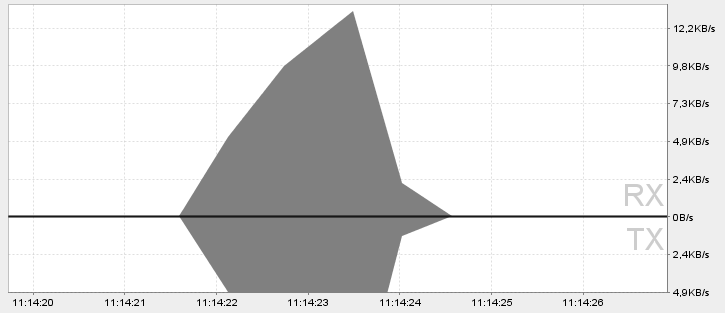
\includegraphics[width=0.45\textwidth]{figures/get_retrofit.png}} \qquad
	\subfloat[GET Request Jersey]{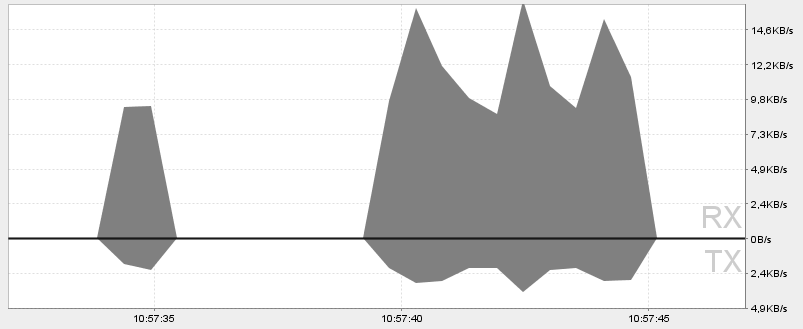
\includegraphics[width=0.45\textwidth]{figures/get_jersey.png}} \qquad
	\subfloat[GET Request Spring for Android]{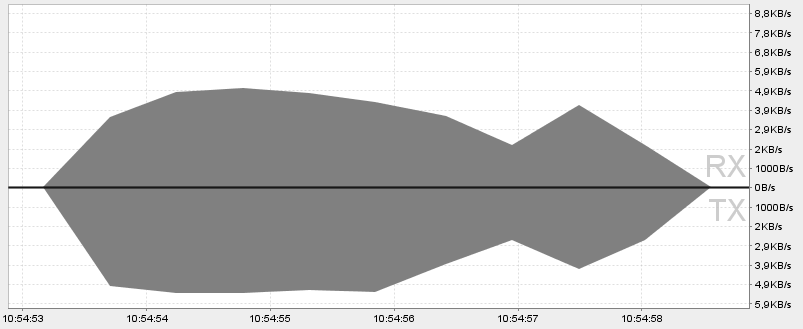
\includegraphics[width=0.45\textwidth]{figures/get_spring.png}} \qquad
	\subfloat[GET Request AndroidAnnotations]{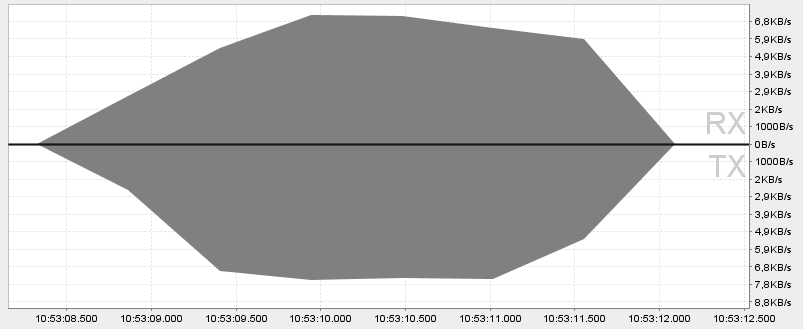
\includegraphics[width=0.45\textwidth]{figures/get_aa.png}}
	\caption{Zeitmessung der GET Requests} 
	\label{getRequests}
\end{figure} 

Die Messung der Zeitdauer für einen POST Request ist aus der Abbildung \ref{postRequests} zu entnehmen. Dabei wurde die Zeit gemessen, bis neu eingegeben Daten um ein neues Kraftwerk anzulegen, erfolgreich zum Server übermittelt wurden. Es konnte dabei festgestellt werden, dass alle Frameworks circa gleich lange benötigen, um die Daten zu übertragen. Spring for Android ist dabei minimal langsamer als die anderen, dies ist aber zu vernachlässigen, da diese Verzögerung keine Auswirkung auf die Usability für einen User hat \cite{meyer:performance}.

\begin{figure} [ht]
	\centering
	\subfloat[POST Request Retrofit]{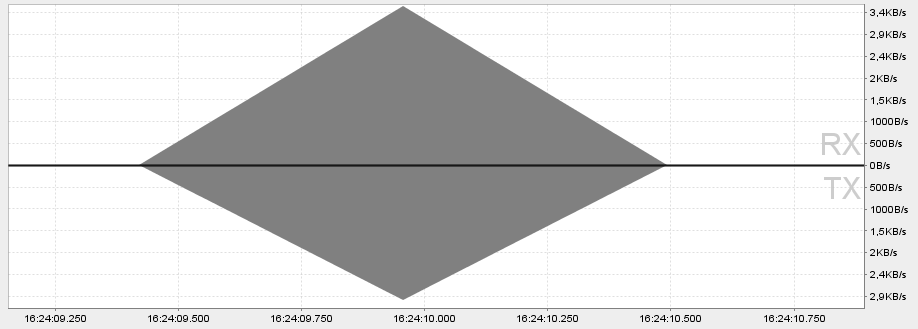
\includegraphics[width=0.45\textwidth]{figures/post_retrofit.png}} \qquad
	\subfloat[POST Request Jersey]{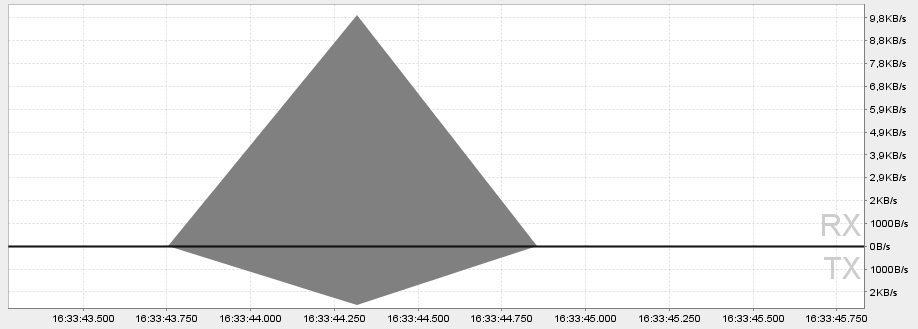
\includegraphics[width=0.45\textwidth]{figures/post_jersey.png}} \qquad
	\subfloat[POST Request Spring for Android]{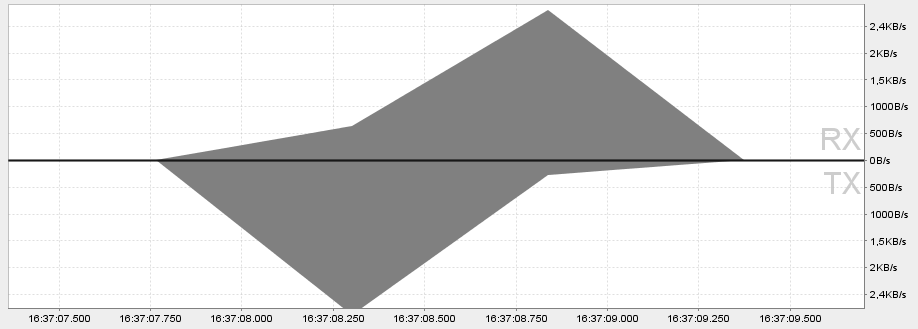
\includegraphics[width=0.45\textwidth]{figures/post_spring.png}} \qquad
	\subfloat[POST Request AndroidAnnotations]{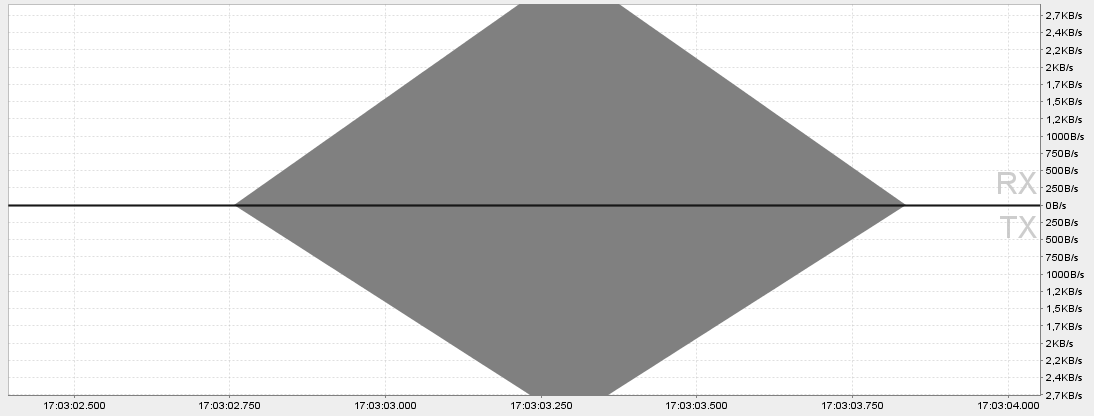
\includegraphics[width=0.45\textwidth]{figures/post_aa.png}}
	\caption{Zeitmessung der POST Requests} 
	\label{postRequests}
\end{figure} 

In der Abbildung \ref{cpuAuslastung} wird die CPU Auslastung der einzelnen Frameworks gegenübergestellt. Aus dieses Abbildung kann entnommen werden, das AndroidAnnotations die CPU am geringsten in Anspruch nimmt und Jersey am stärksten. Bei der Benutzung der Apps ist auch festzustellen, dass AndroidAnnotations und Retrofit am schnellsten arbeiten und eine flüssige Bedienung der Anwendung möglich ist. Jersey ist des öfteren langsam und hat kleine Ruckler währende der Bedienung.  

\begin{figure} [ht]
	\centering
	\subfloat[CPU Auslastung Retrofit]{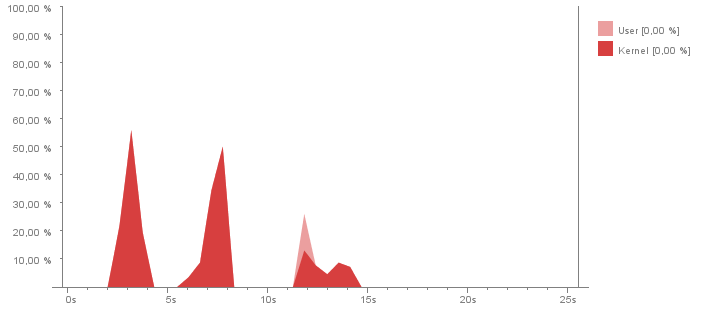
\includegraphics[width=0.45\textwidth]{figures/cpu_retrofit.png}} \qquad
	\subfloat[CPU Auslastung Jersey]{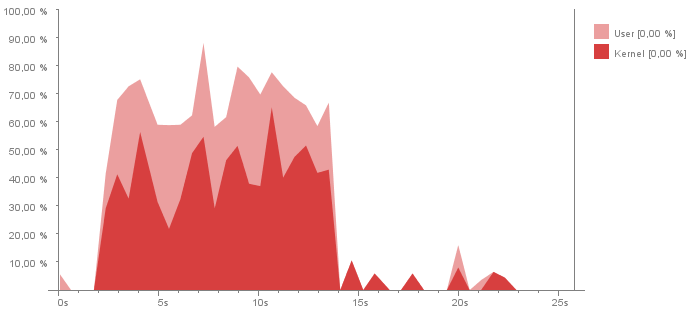
\includegraphics[width=0.45\textwidth]{figures/cpu_jersey.png}} \qquad
	\subfloat[CPU Auslastung Spring for Android]{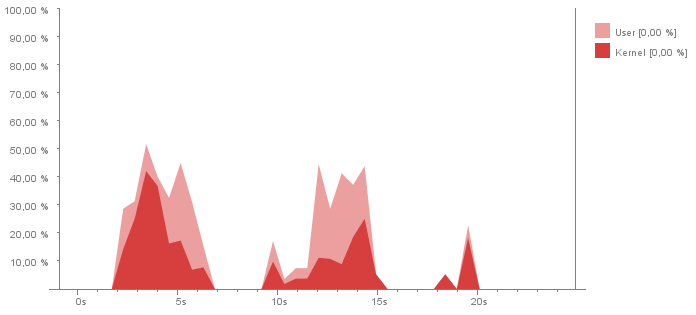
\includegraphics[width=0.45\textwidth]{figures/cpu_spring.png}} \qquad
	\subfloat[CPU Auslastung Request AndroidAnnotations]{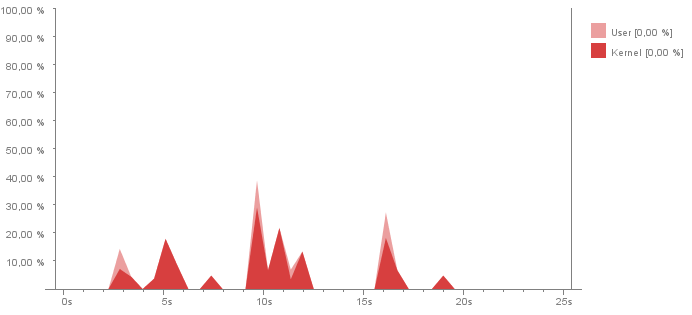
\includegraphics[width=0.45\textwidth]{figures/cpu_aa.png}}
	\caption{CPU Auslastung} 
	\label{cpuAuslastung}
\end{figure} 

\textbf{Speicherplatz}\\


\begin{landscape}
% m{3.5cm}|m{4.5cm}|m{4.5cm}|m{4.5cm}|m{4.5cm}
\renewcommand{\arraystretch}{1.3}
\begin{longtable}{ m{3.5cm}|m{4.5cm}|m{4.5cm}|m{4.5cm}|m{4.5cm}}
	%	>{\centering \arraybackslash}m{3.5cm}|
	%	>{\centering \arraybackslash}m{4.5cm}|
	%	>{\centering \arraybackslash}m{4.5cm}|
	%	>{\centering \arraybackslash}m{4.5cm}|
	%	>{\centering \arraybackslash}m{4.5cm}}

      \caption{Gegenüberstellung der Frameworks} \\
	  \label{tableVergleich}	 
	  
	    & \textbf{Retrofit} & \textbf{Jersey} & \textbf{Spring for Android}  & \textbf{AndroidAnnotations}  \\  \hhline{=====}
	   \multicolumn{5}{c}{\textbf{Entwicklungskultur}} \\ \hhline{=====}
	  \textbf{Lizenz} &
	  Apache License Version 2.0 & CDDL Version 1.1 \newline GPL Version 2 & 
	  Apache License Version 2.0 & 
	  Apache License 2.0 \newline CDDL \\ \hline
	  \textbf{aktive Community} & Ja & Ja & Ja & Ja\\ \hline
	  \textbf{Dokumentation} & grundlegend & gut & gut  & gut \\ \hline 
		  \textbf{Codebeispiele} &  Ja  & nicht speziell für Android & Ja & Ja\\ \hhline{=====}
	  
	  \multicolumn{5}{c}{\textbf{Implementierung}} \\ \hhline{=====}
	  \textbf{Einbindung} & leicht & problematisch & leicht & leicht \\ \hline
	  \textbf{HTTP-Verben} & GET, POST, PUT, DELETE, HEAD & GET, POST, PUT, DELETE, HEAD, OPTIONS  & GET, POST, PUT, DELETE, HEAD, OPTIONS & GET, POST, PUT, DELETE, HEAD, OPTIONS \\ \hline
	  \textbf{HTTP-Header} & erweiterbar & erweiterbar & erweiterbar & erweiterbar \\ \hline
	  \textbf{unterstützte\newline Medientypen} & alle möglichen, wenn Konverter für Typ vorhanden ist & alle möglichen, wenn Konverter für Typ vorhanden ist & alle möglichen, wenn Konverter für Typ vorhanden ist & alle möglichen, wenn Konverter für Typ vorhanden ist \\ \hline
	  \textbf{URL veränderbar} & Ja & Ja & Ja & Ja  \\ \hline
	  \textbf{HATEOAS Konzept} & Nein & Ja & mithilfe von Spring HATEOAS & ohne Annotations und mithilfe von Spring HATEOAS \\ \hline 
	  \textbf{Error-Handling} \\ \hhline{=====}
	  \multicolumn{5}{c}{\textbf{Performance und Speicherplatz}} \\ \hhline{=====}
	  
	  \textbf{GET Request} & \textasciitilde3s & \textasciitilde12s  & \textasciitilde5s & \textasciitilde3.5s\\ \hline
	  
	  \textbf{POST Request} & \textasciitilde1s &  \textasciitilde1s & \textasciitilde1.5s & \textasciitilde1s \\ \hline
	  
	  \textbf{CPU Auslastung} & max. \textasciitilde55\%  & max. \textasciitilde87\% & max. \textasciitilde52\% & max. \textasciitilde40\%\\ \hline
	  \textbf{belegter RAM} & max. 9.11 MB & max. 11.83 MB & max. 8.93 MB & max 7.02 MB \\ \hline
	  \textbf{.apk-Größe} & 1.70 MB & 2.58 MB & 1.69 MB & 1.44 MB \\ \hhline{=====}

	   \multicolumn{5}{c}{\textbf{Erweiterte Technische Fähigkeiten}} \\ \hhline{=====}
	   \textbf{Sicherheit} & \\ \hline
	   \textbf{andere Protokolle außer HTTP} & \\ \hline
	   \textbf{asynchroner Nachrichtenaustausch} & Ja & Ja & Ja & Ja \\ \hline
	   \textbf{ACID-Eigenschaften} & Ja & Ja & Ja & Ja \\ \hline
	   \textbf{Server Implementierung} & Nein & Ja &  Spring Framework & Nein (eventuell Spring Framework) \\ \hline
	   \textbf{zusätzliche Dienste} & Nein & Nein & Nein & Ja \\ \hline
 
\end{longtable}
\end{landscape}

\section{Persönliches Fazit zu den Frameworks}
Es folgt nun ein kurzer Persönlicher Eindruck zu den Frameworks, wo traten Probleme während der Implementierung auf oder welche Aspekte positiv aufgefallen sind.
\\\\
\textbf{Jersey}
\\\\
\textbf{Retrofit}
\\\\
\textbf{Spring for Android}
\\\\
\textbf{AndroidAnnotations}
\\\\